\section{Layer representations}

Let $\cl = (g,h)$ a neural network layer, where $g: I \rightarrow O$ is its linear part, $h : O \rightarrow O$ is its activation function, $I$ and $O$ are its input and output spaces, which are tensor spaces. 

\subsection{Neural interpretation of tensor spaces}

Recall from \defref{def:tensor} that a tensor space has been defined such that its canonical basis is a cartesian product of canonical bases of vector spaces. Let $I = \bigotimes_{k=1}^p \bbv_k$ and $O =  \bigotimes_{l=1}^q \bbu_l$.
Their canonical bases are denoted $\vv_k = (\vv_k^1, \ldots, \vv_k^{n_k})$ and $\uu_l = (\uu_l^1, \ldots, \uu_l^{n_l})$.

\begin{remark}
Note that a tensor space is isomorph to the signal space defined over its canonical basis.
\end{remark}

More precisely, we have the following relation.

\begin{lemma}\textbf{Relation between tensor and signal spaces}\\
Let $\bbv$, $\bbu$ vector spaces, and $\vv$, $\uu$ their canonical bases. Let $\bbt$ a tensor space. $\otimes$ and $\times$ denote tensor and cartesian products. Then,
\begin{enumerate}[label=(\roman*)]
  \item $\bbv \cong \cs(\vv)$
  \item $\bbv \otimes \bbu \cong \cs(\vv \times \uu)$
  \item $\bbv \otimes \bbt \cong \cs_{\bbt}(\vv)$
\end{enumerate}
where $\cs_{\bbt}$ are signals taking values in $\bbt$ (and $\cs$ are real-valued signals).
\label{lem:relts}
\end{lemma}
\begin{proof}
\begin{enumerate}[label=(\roman*)]
  \item Given $x \in \bbv$, define $\widetilde{x} \in \cs(\vv)$ such that $\forall i, \widetilde{x}[\vv^i] = x[i]$. The mapping $x \mapsto \widetilde{x}$ is a linear isomorphism. \label{enum:li}
  \item $\widetilde{x}[\vv^i, \uu^j] = x[i,j]$
  \item $\widetilde{x}[\vv^i] = x[i,:,\ldots,:]$
\end{enumerate}
\end{proof}

Let $d \le n_k$ and $e \le n_l$. Define $V$ and $U$ as the cartesian products $V = \bigtimes_{k=1}^d \vv_k$ and $U = \bigtimes_{l=1}^e \uu_l$. Thanks to \lemref{lem:relts}, we can identify the input and output spaces as $I = \cs(V) \otimes \bigotimes_{k=d+1}^p \bbv_k$ and $O = \cs(U) \otimes \bigotimes_{l=e+1}^q \bbu_l$. As $\cs(\vv) \otimes \bbt = \cs_{\bbt}(\vv)$, an object of $V$ or $U$ can be interpreted as the representation of a \emph{neuron} which can take multiple values.

%\paragraph{A convenient simplification}
\vspace{10pt}
In what follows, without loss of generality, we will make the simplification that a neuron can only take a single value (we don't consider input channels and feature maps yet). We'll thus consider that $I = \cs(V)$ and $O = \cs(U)$, where $V$~is the set of \emph{input neurons}, and $U$ is the set of \emph{output neurons}.

%\subsection{Graph representations}
\subsection{Propagational interpretation}

Let $\cl = (g,h)$, recall that $g: \cs(V) \rightarrow \cs(U)$ is characterized by a connectivity matrix $W$ such that, $g(x) = Wx$.

\begin{remark}Using the mapping defined in the proof of \lemref{lem:relts}, for notational conveniency, we'll abusively consider $x$ as a vector (enventually reshaped from a tensor), and $W$ as an object of a binary tensor product for its indexing (\ie $W[u,v] := W[i,j]$ where $u = \uu^i$ and $v = \vv^j$).
\end{remark}

% Define bipartite graph here?

\begin{definition}\textbf{Propagation graph}\\
The \emph{propagation graph} $P = \langle (V, U), E_P \rangle$ of a layer $\cl = (W,h)$ is the bipartite graph that has the connectivity matrix $W$ for bipartite adjacency matrix.
\end{definition}

An example is depicted on \figref{fig:pgraph}.

\begin{figure}[H]
\centering
\begin{tikzpicture}
\draw (0,0) -- (4,0) -- (4,4) -- (0,4) -- (0,0);
\node at (2,2){placeholder};
\end{tikzpicture}
\caption{A propagation graph}
\label{fig:pgraph}
\end{figure}

% This representation stresses out the fact that every layer is in fact a partially connected layer.
% To say in weight sharing scheme

The propagation graph defines an input topological space~$\ct_V$, and an output topological space~$\ct_U$.

\begin{definition}\textbf{Topological space}\\
A \emph{topological space} is a pair $\ct = (X, \co)$, where $X$ is a set of points, $\co$ is a set of sets that is closed under intersection (the \emph{open sets}), and such that every point $x \in X$ is associated with a set $\cn_x \in \co$, called its \emph{neighborhood}.
\end{definition}

Hence, the \emph{neural topologies} $\ct_V$ and $\ct_U$ are defined as
\begin{enumerate}
\item $\ct_V = (V, \co(U))$, with $\forall v \in V, \cn_v = \{u \in U, v \overset{P}\sim u \}$
\item $\ct_U = (U, \co(V))$, with $\forall u \in U, \cn_u = \{v \in V, v \overset{P}\sim u \}$
\end{enumerate}

In particular, given an output neuron $u \in U$, a neighborhood $\cn_u$ is also called a \emph{receptive field}, that we denote $\ccr_u$.

\subsection{Graph representation of the input space}

Let's consider that the input neurons $V$ have a (possibly edge-less) graph structure $\gve$. We define an edge-constrained layer as follows.

\begin{definition}\textbf{Edge-constrained layer}\\
A layer $\cl: \gve \rightarrow U$, is said to be \emph{edge-constrained} (EC) if:
\begin{enumerate}
  \item There is a one-to-one correspondence $\pi: V_\pi \rightarrow U$, where $V_\pi \subset V$.
  \item Given an output neuron $u$, an input neuron $v$ is in its receptive field, if and only if, $v$ and the $\pi$-fiber of $u$ are connected in $G$,\\
  \centerline{\ie $\forall u \in U, v \in \ccr_u \Leftrightarrow v \overset{E}\sim \pi^{-1}(u) $}
\end{enumerate}
\end{definition}

Note that (EC) convolutions are (EC) layers. We have the following characterization.

\begin{proposition}\textbf{(EC) Characterization with receptive fields}\\
Let a layer $\cl: V \rightarrow U$, $V_\pi \subset V$, and a one-to-one correspondence $\pi: V_\pi \rightarrow U$. There exists a graph $\gve$ for which $\cl$ is (EC), if and only if, the receptive fields are \emph{intertwined} (\ie $\forall a,b \in V_\pi, a \in \ccr_{\pi(b)} \Leftrightarrow b \in \ccr_{\pi(a)} $).
\end{proposition}
\begin{proof}
\begin{enumerate}
  \item[($\Rightarrow$)] Thanks to $a \in \ccr_{\pi(b)} \Leftrightarrow a \overset{E}\sim b \Leftrightarrow b \in \ccr_{\pi(a)}$
  \item[($\Leftarrow$)] If the receptive fields are intertwined, then the relation defined as\\ $a \sim b \Leftrightarrow a \in \ccr_{\pi(b)}$ is symmetric, and thus can define an edge set.
\end{enumerate}
\end{proof}

Therefore, any layer that has its receptive fields intertwined, admits an \emph{underlying} graph structure. For example, a $2$-d convolution operator can be rewritten as an (EC*) convolution on a lattice graph, and as an (EC) convolution on a grid graph.

\figref{fig:upgraph} depicts an underlying graph and its corresponding propagation graph.

\begin{figure}[H]
\centering
\begin{tikzpicture}
\draw (0,0) -- (4,0) -- (4,4) -- (0,4) -- (0,0);
\node at (2,2){placeholder};
\draw (5,0) -- (5,4) -- (9,4) -- (9,0) -- (5,0);
\node at (7,2){placeholder};
\end{tikzpicture}
\caption{Underlying graph Vs Prop graph}
\label{fig:upgraph}
\end{figure}

\subsection{General representation with weight sharing}

Weight sharing refers to the fact that some parameters of the connectivity matrix $W$ are equal, and stay equal after each learning iteration. In other words they are tied together. From a propagational point of view, this amounts to label the edges of the propagation graph $P$ with weights, where weights can be used multiple times to label these edges. Supposed $W$ is of shape $m \times n$ and there are $\omega$ weights in the kernel used to label the edges. Given a input neuron $i$ and an output neuron $j$, the edge labelling can be expressed as:
\begin{gather}
%W[i,j] = \theta[h] = \theta^T S[:,i,j]
W[j,i] = \theta[h] = \theta^T a \label{eq:alloc}
\end{gather}
where $\theta$, the weight kernel, is a vector of size $\omega$ and $a$ is a one-hot vector (full of $0$s except for one $1$) of size $\omega$ with a $1$ at the index $h$ corresponding to the weight that labels the edge $i \sim j$ ; or $a$ is the \emph{zero} vector in case $i \nsim j$.

This equation \eqref{eq:alloc} can be rewritten as a tensor contraction under Einstein summation convention, by noticing that $a$ depends on $i,j$ and by defining a tensor $S$ such that $a = S[:,i,j]$, as follows:
\begin{gather}
W_{ij} = \theta_k S^k \h{0}_{ij}
\end{gather}
Therefore, the linear part of $\cl$ can be rewritten as:
\begin{gather}
g(x)_j = \theta_k S^k \h{0}_j \h{0}^i x_i
\end{gather}

If we consider that the layer $\cl$ is duplicated with input channels and feature maps, then $\theta$, $x$ and $g(x)$ become tensors, denoted $\Theta$, $X$ and $g(X)$. Usually, for stochastic gradient descent, $X$ and $g(X)$ are also expanded with a further rank corresponding to the batch size and we obtain:
\begin{gather}
g(X) = \Theta S X
\text{ where } \begin{cases} W_{pq}\h{0}^{ij} = \Theta_{pq}\h{0}^k S_k\h{0}^{ij} \\ g(X)_{jq}\h{0}^b = W_{jq}\h{0}^{ip} X_{ip}\h{0}^{b} \end{cases} \label{eq:ternary}
\end{gather}

\begin{table}[H]
  \centering
\begin{tabular}{ccl}
  index & size & description\\
  \hline
  $i$ & $n$ & input neuron\\
  $j$ & $m$ & output neuron\\
  $p$ & $N$ & input channel\\
  $q$ & $M$ & feature map\\
  $k$ & $\omega$ & kernel weight\\
  $b$ & $B$ & batch instance
\end{tabular}
\caption{Table of indices}
\label{tab:ind}
\end{table}

\begin{remark}
Note that the expression $\Theta S X$ is written regardless of the ordering of the tensors ranks and is defined by index juggling. %Therefore, it is an associative and commutative ternary operation between $\Theta$, $S$  and $X$, which contracts them along the input ranks (neurons and channels) and the weight rank.
\end{remark}

Also, note that it is associative and commutative. This can be seen by the index symmetry of \eqref{eq:comm}, which rewrites~\eqref{eq:ternary}, and where the sum symbols~$\Sigma$ and scalar values commute:

\begin{gather}
\Theta SX[j,q,b] = \displaystyle \sum_{k=1}^\omega \sum_{p=1}^P \sum_{i=1}^n \Theta[k,p,q] \h{2} S[k,i,j] \h{2} X[i,p,b] \label{eq:comm}
\end{gather}

We call $S$ the \emph{weight sharing scheme} \citep{vialatte2017learning} of the layer $\cl$.

\begin{definition}\textbf{Ternary representation}\\
The \emph{ternary representation} of a layer $\cl: X \mapsto Y$, with activation function~$h$, is the equation $Y = h\left(\Theta S X\right)$, as defined in $\eqref{eq:ternary}$, where~$\Theta$ is the \emph{weight kernel}, and~$S$ is called the \emph{weight sharing scheme}.
\end{definition}

\begin{remark}
In $\eqref{eq:alloc}$, we defined $a = S[:,i,j]$ as a one-hot vector when $i \sim j$, as its role is to select a weight in $\theta = \Theta[p,q,:]$. However, $a$ can also do this selection \emph{linearly}, so in fact it is not necessarily a one-hot vector.
\end{remark}

\figref{fig:ternary} depicts an example of how the equation \eqref{eq:ternary} labels the edges of $P$.
\begin{figure}[H]
  \begin{center}
    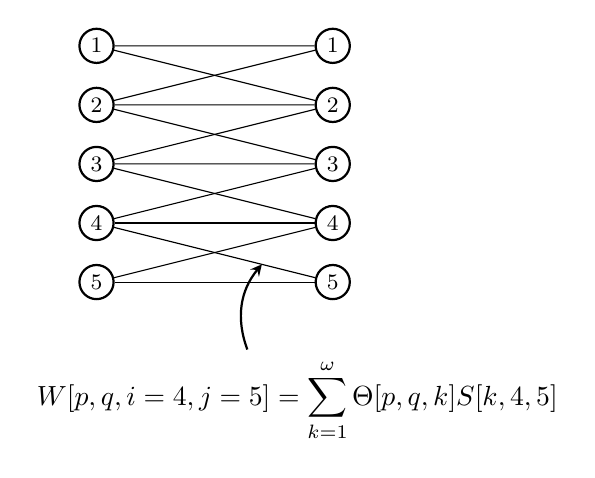
\begin{tikzpicture}[scale=1.5]
      \tikzstyle{every node} = [draw, circle, thick, inner sep = 2pt]
      
        \foreach \y in {0,...,4}{
          \pgfmathtruncatemacro{\yplusone}{5 - \y}

          \node(a\y) at (0,.5*\y) {\footnotesize\yplusone};
      }
        \foreach \y in {0,...,4}{
          \pgfmathtruncatemacro{\yplusone}{5 - \y}
                  
          \node(\y) at (2,.5*\y) {\footnotesize\yplusone};
      }
      \path
      (a0) edge (0)
      (a0) edge (1);
      \path
      (a1) edge (0)
      (a1) edge (1)
      (a1) edge (2);
      \path
      (a2) edge (1)
      (a2) edge (2)
      (a2) edge (3);
      \path
      (a3) edge (2)
      (a3) edge (3)
      (a3) edge (4);
      \path
      (a4) edge (3)
      (a4) edge (4);

      \tikzstyle{every node} = []
      \node(label) at (1.7,-1) {$W[p,q,i=4,j=5] = \displaystyle{\sum_{k=1}^{\omega}{\Theta[p,q,k] S[k,4,5]}}$};
      \path[>=stealth, ->, thick]
      (label) edge[bend left] (1.4,0.15);
    \end{tikzpicture}
  \end{center}
  \caption{Example of a propagation graph $P$ for a given input channel $p$ and feature map $q$. The edge $4 \sim 5$ is labelled with a linear combination of kernel weights from $\Theta[p,q,:]$. In the usual case, $S[k,4,5]$ is a one-hot vector that selects a single kernel weight: $\exists h, W[p,q,4,5] = \Theta[p,q,h]$.}
  \label{fig:ternary}
\end{figure}

The ternary representation uncouples the roles of $\Theta$ and $S$ in $W$, and is the most general way of representing any kind of partially connected layer with weight sharing.
